\documentclass[10pt]{article}
\usepackage[polish]{babel}
\usepackage[utf8]{inputenc}
\usepackage[T1]{fontenc}
\usepackage{amsmath}
\usepackage{amsfonts}
\usepackage{amssymb}
\usepackage[version=4]{mhchem}
\usepackage{stmaryrd}
\usepackage{graphicx}
\usepackage[export]{adjustbox}
\graphicspath{ {./images/} }

\title{GIMNAZJUM }

\author{}
\date{}


\begin{document}
\maketitle
\begin{enumerate}
  \item Dane są nieujemne liczby wymierne \(a\) i \(b\).
\end{enumerate}

Udowodnij, że jeżeli suma \(\sqrt{a}+\sqrt{b}\) jest wymierna, to każda z liczb \(\sqrt{a}, \sqrt{b}\) jest wymierna.\\
2. Oblicz kąty w trójkącie \(A B C\) wiedząc, że prosta \(C D\) jest styczną do okręgu, odcinki \(C B\) i \(B D\) mają jednakową długość oraz kąt \(C D B\) ma \(40^{\circ}\).\\
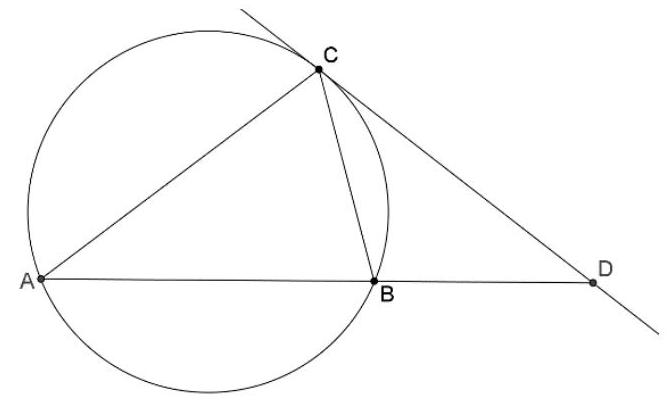
\includegraphics[max width=\textwidth, center]{2024_11_21_92e4b017f3ebdb44cbd9g-1}\\
3. Zdecyduj, czy liczba \(\begin{array}{cc}\frac{1}{1+\frac{1}{2+\frac{1}{3+}}} & +\frac{1}{2+\frac{1}{3+\frac{1}{4+}}} \text { jest większa czy mniejsza niż } 1 . \\ \ddots & \ddots \\ +\frac{1}{50} & +\frac{1}{50}\end{array}\)

\section*{LICEUM}
\begin{enumerate}
  \item Zbadaj, czy istnieje ciąg arytmetyczny, w którym występują wyrazy \(\sqrt{2}, \sqrt{3}, \sqrt{5}\) (niekoniecznie jako trzy kolejne).
  \item Okrąg \(o_{1}\) przechodzi przez środek okręgu \(o_{2}\) i przecina go w punktach A i B. Udowodnij, że cięciwa AB i odcinek stycznej AC mają jednakową długość.
  \item Sprawdź, która liczba jest większa: \(8^{40}\) czy \(5^{40}+6^{40}\).\\
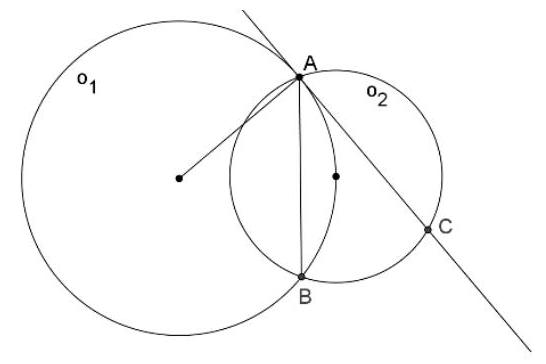
\includegraphics[max width=\textwidth, center]{2024_11_21_92e4b017f3ebdb44cbd9g-1(1)}
\end{enumerate}

\end{document}